\documentclass{article}

\usepackage{graphicx}
\usepackage{tikz}
\usepackage{tikzsymbols}
\usetikzlibrary{calc,patterns,shapes.geometric}
\pagestyle{empty}
\usepackage[margin=0pt]{geometry}
\geometry{papersize={14in,12in}}

\def\centerarc[#1](#2)(#3:#4:#5){\draw[#1] ($(#2)+({#5*cos(#3)},{#5*sin(#3)})$) arc (#3:#4:#5);}

\begin{document}
	\begin{figure}
		\centering
		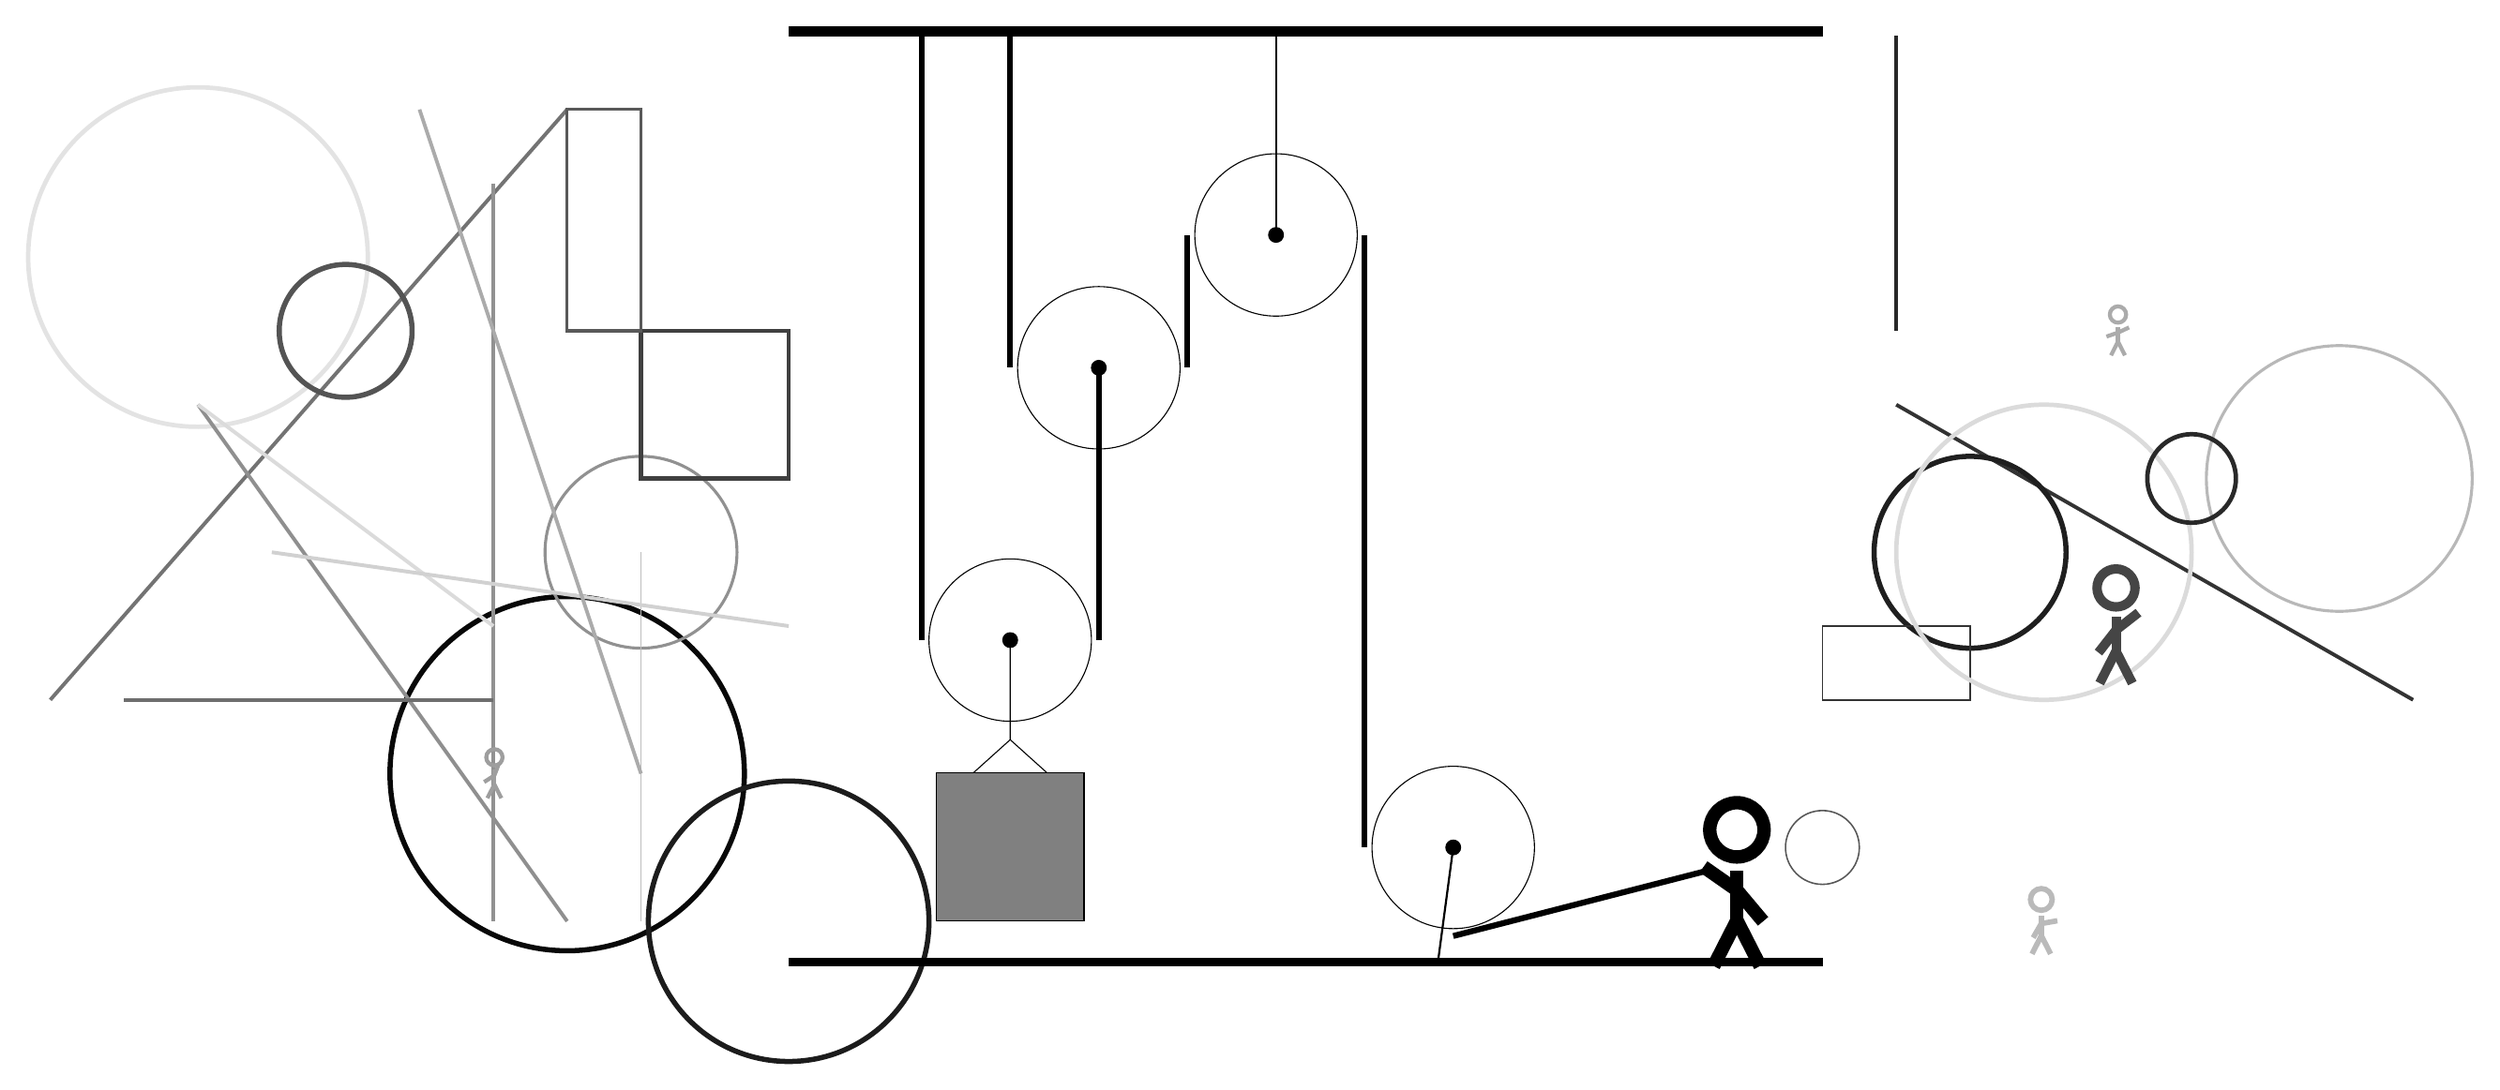
\begin{tikzpicture}
			%%%%% START %%%%%
			
			\draw[fill=black] (-2, 9) rectangle (12, 9.125);
			
			\draw (1, 0.81) circle (1.1);
			\draw[fill=black] (1, 0.81) circle (0.1);
			
			\draw (2.2, 4.5) circle (1.1);
			\draw[fill=black] (2.2, 4.5) circle (0.1);
			
			\draw (4.6, 6.3) circle (1.1);
			\draw[fill=black] (4.6, 6.3) circle (0.1);
			\draw[thick] (4.6, 6.3) -- (4.6, 9);
			
			\draw (7.0, -2) circle (1.1);
			\draw[fill=black] (7.0, -2) circle (0.1);
			\draw[thick] (7.0, -2) -- (6.8, -3.5);
			
			\draw [line width=0.6mm, color=black!11](-10, 6) circle (2.3);
			
			\draw [line width=0.7mm, color=black!97](-5, -1) circle (2.4);
			\draw[line width=0.5mm, color=black!55](-5, 8) -- (-12, 0);
			\draw[line width=0.5mm, color=black!44](-5, -3) -- (-10, 4);
			\draw[line width=0.5mm, color=black!43](-6, 7) -- (-6, -3);
			\node[line width=0.4mm, color=black!38] at (-6, -1) {\Strichmaxerl[3][33][69]};
			\draw [line width=0.4mm, color=black!43](-4, 2) circle (1.3);
			
			\draw[line width=0.5mm, color=black!80](13, 4) -- (20, 0);
			\draw [line width=0.7mm, color=black!88](14, 2) circle (1.3);
			\draw[line width=0.2mm, color=black!80] (12, 0) rectangle (14, 1);
			\draw [line width=0.7mm, color=black!89](-2, -3) circle (1.9);
			
			\draw [line width=0.2mm, color=black!66](12, -2) circle (0.5);
			\draw [line width=0.4mm, color=black!28](19, 3) circle (1.8);
			\draw[line width=0.5mm, color=black!57](-6, 0) -- (-11, 0);
			\draw[line width=0.2mm, color=black!26] (-4, -3) rectangle (-4, 2);
			\node[line width=0.2mm, color=black!27] at (15, -3) {\Strichmaxerl[4][60][10]};
			
			\draw [line width=0.6mm, color=black!14](15, 2) circle (2.0);
			\node[line width=0.3mm, color=black!33] at (16, 5) {\Strichmaxerl[3][19][25]};
			\draw[line width=0.5mm, color=black!14](-6, 1) -- (-10, 4);
			\draw[line width=0.6mm, color=black!75] (-2, 3) rectangle (-4, 5);
			\draw[line width=0.5mm, color=black!18](-2, 1) -- (-9, 2);
			\node[line width=0.3mm, color=black!73] at (16, 1) {\Strichmaxerl[7][52][38]};
			\draw [line width=0.7mm, color=black!67](-8, 5) circle (0.9);
			\draw[line width=0.4mm, color=black!65] (-4, 8) rectangle (-5, 5);
			\draw [line width=0.6mm, color=black!84](17, 3) circle (0.6);
			\draw[line width=0.5mm, color=black!33](-7, 8) -- (-4, -1);
			\draw[line width=0.5mm, color=black!84](13, 5) -- (13, 9);
			
			\draw (1, 0.81) -- (1, -0.54) -- (0.5, -0.99) -- (1.5, -0.99) -- (1, -0.54);
			\draw[fill=black!50] (0, -0.99) rectangle (2, -2.99);
			\draw[line width=0.8mm] (-0.2, 9) -- (-0.2, 0.81);
			\centerarc[line width=0.8mm](1, 0.81)(180:360:1.2000000000000002);
			\draw[line width=0.8mm](2.2, 0.81) -- (2.2, 4.5);
			\draw[line width=0.8mm] (1.0, 9) -- (1.0, 4.5);
			\centerarc[line width=0.8mm](2.2, 4.5)(180:360:1.2000000000000002);
			\draw[line width=0.8mm](3.4, 4.5) -- (3.4, 6.3);
			\centerarc[line width=0.8mm](4.6, 6.3)(0:180:1.2000000000000002);
			\draw[line width=0.8mm] (5.8, 6.3) -- (5.8, -2);
			\centerarc[line width=0.8mm](7.0, -2)(0:90:-1.2000000000000002);
			\draw[line width=0.8mm](7.0, -3.2) -- (10.5, -2.3);
			
			\node at (10.8, -2.5) {\Strichmaxerl[10][-35][-50]};
			
			\draw[fill=black] (-2, -3.5) rectangle (12, -3.6);
			
			%%%%% END %%%%%
		\end{tikzpicture}
	\end{figure}	
\end{document}